\normalfalse \difficiletrue \tdifficilefalse
\correctionfalse

%\UPSTIidClasse{11} % 11 sup, 12 spé
%\newcommand{\UPSTIidClasse}{12}

\exer{Mouvement RT -- RSG  $\star\star$ \label{CIN:01:B2:12:09}}
\setcounter{question}{0}\marginnote{\xpComp{CIN}{01}}%\UPSTIcompetence{B2-12}
\index{Compétence B2-12}\index{Compétence CIN-01}
\index{Mécanisme à 1 rotations, 1 translation et RSG}
\ifcorrection
\else
\marginnote{\textbf{Pas de corrigé pour cet exercice.}}
\fi

\ifprof
\else
Soit le mécanisme suivant. On a $\vect{IA}=R\vect{j_0}$ et $\vect{AB}=\lambda(t)\vect{i_1}$. De plus $R=\SI{15}{mm}$.
\begin{marginfigure}
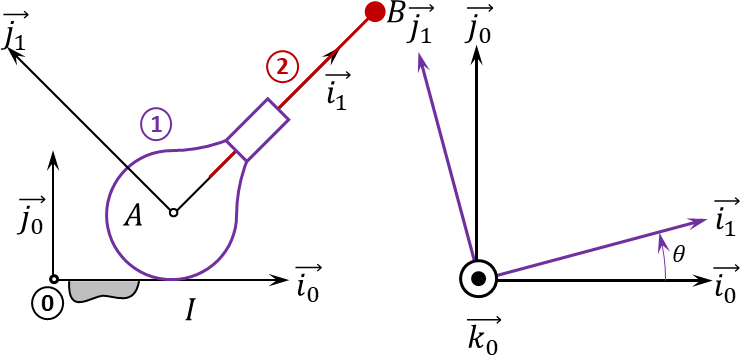
\includegraphics[width=\linewidth]{09_RT_RSG_01}
\end{marginfigure}
\fi


\question{Tracer le graphe des liaisons.}
\ifprof
\else
\fi


\question{Retracer le schéma cinématique pour $\theta(t)=0\,\text{rad}$ et $\lambda(t)=\SI{20}{mm}$. On notera $I_1$ le point de contact entre \textbf{0} et \textbf{1}.}
\ifprof
\else
\fi

\question{Retracer le schéma cinématique pour $\theta(t)=\dfrac{\pi}{2}\,\text{rad}$ et $\lambda(t)=\SI{30}{mm}$. On notera $I_2$ le point de contact entre \textbf{0} et \textbf{1}. On précisera la position des points $I_{0,0}$ et $I_{0,1}$, points résultants de la rupture de contact lors du passage de $\theta(t)$ de 0 à $\dfrac{\pi}{2}$.}
\ifprof
\else
\fi





\ifprof
\else

\marginnote{Corrigé  voir \ref{CIN:01:B2:12:09}.}

\fi